In the last few decades, we are witnessing fast and numerous shifts from dedicated single object observations to massive all-sky surveys producing hundreds or even thousands of unbiased observations in a single telescope pointing. Along with the complexity of data acquisition and storage, new challenges and problems involving data reduction arose, requiring dedicated computer power to reduce acquired data. The reduction challenges span from timely, almost real-time reduction requirements, to complex, computationally demanding processes that try to take into account as many telescopically and observationally induced biases as possible. Some of those processes will be discussed in the following sections discussing a specific survey.

This thesis shows a few cases of synergies of such vastly different data sets and at the same time points to a necessity of having knowledge about the automatic processing pipelines that produced final products. Something that is quite often blindly overlooked by users.

The primary sources of data for our studies are the following three stellar surveys producing information about the stars' brightness, composition, distance, kinematics and many additional parameters that can be inferred from the observed quantities.

\begin{figure}
	\centering
	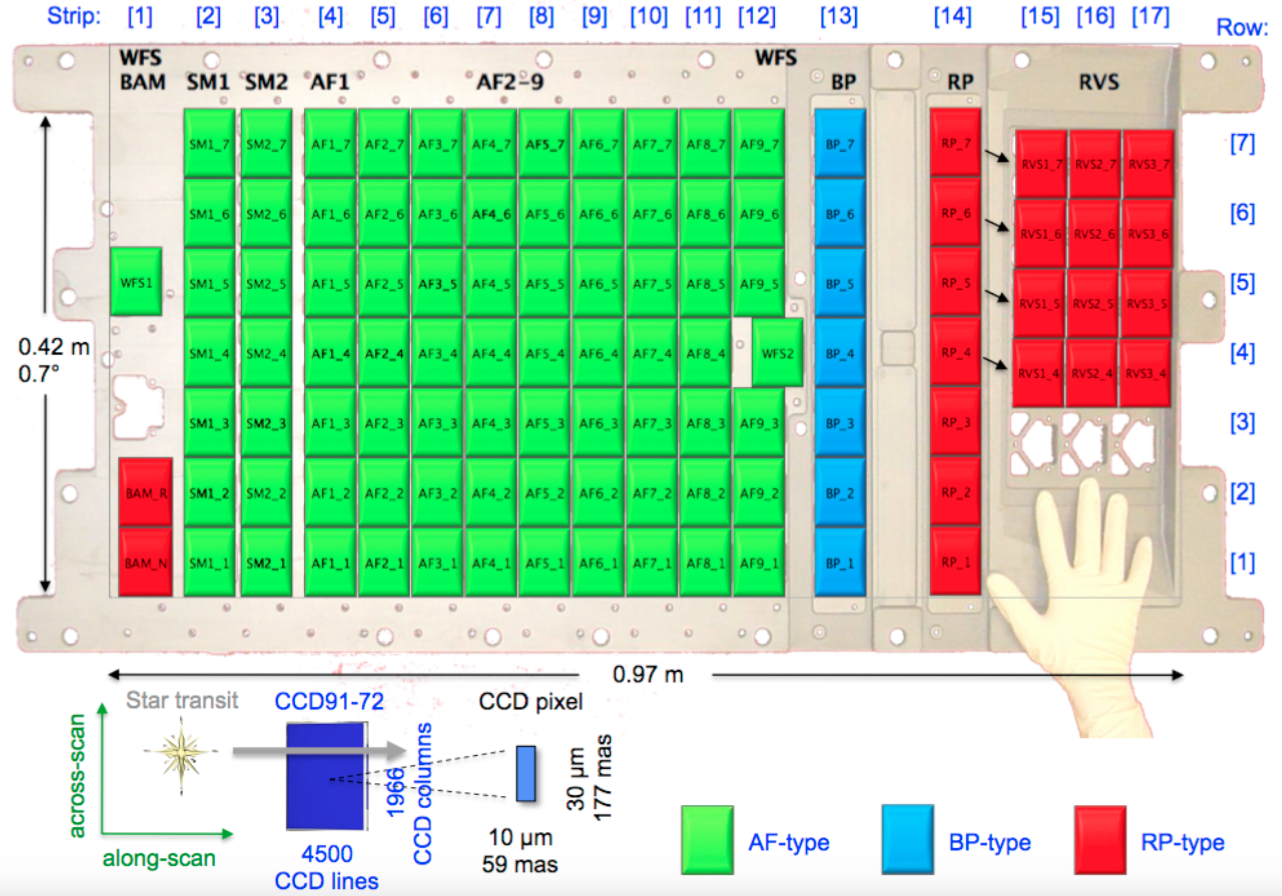
\includegraphics[width=\columnwidth]{gaia_ccd.png}
	\caption{Size comparison and spatial arrangement of the CCD detectors in the \G\ focal plane. Image credit: \citet{2016A&A...595A...1G}.}
	\label{fig:gaia_ccd}
\end{figure}

\section{\G\ space mission}
\label{sec:gaia_data}
\G\ is the one-billion-star surveyor of the European Space Agency (ESA). It has been continuously scanning the sky since July 2014 from its designated location close to the second Lagrange point of the Sun-Earth/Moon system. \G aims to map the entire sky, down to magnitude $\sim20.7$, and to collect micro-arcsecond-level astrometry and milli-magnitude-level photometry for the brightest 1,000+ million stars as well as medium-resolution spectroscopy for mainly radial-velocity determination of the brightest subset of $\sim150$ million objects. 

The \G\ scanning of the sky is composed of two independent, superimposed motions: rotation around the spacecraft spin axis with a period of 6 hours plus a slow, 63 day period precession of the spin axis around the Solar direction at a fixed Solar-aspect angle of $45^\circ$. Over the nominal five-year mission, \G\ has completed $29$ of these precession periods, leading to an optimally uniform sky coverage with, on average, $\sim70$ astrometric and photometric transits across the focal plane (and $\sim40$ for the spectroscopic instrument). In the extended mission phase that started in July 2019, a similar scanning law is being employed but with a reversed precession direction during the first year. Passage of a star through the focal plane is called a field-of-view transit. During each transit, \G\ collects instantaneous, so-called epoch data of each object. Publication of all epoch data is scheduled (see Table \ref{tab:gaia_drs} for the final data release.

\begin{table}
	\centering
	\caption{Past and future predicted release dates of \G\ data and products.}
	\begin{tabular}{c c}
		\hline
		Release designation & Date \\ 
		\hline
		\G\ DR1 & 14 September 2016 \\
		\G\ DR2 & 25 April 2018 \\
		\G\ EDR3 & 2$^{nd}$ half of 2020 or later \\
		\G\ DR3 & postponed into late 2021 or later \\
		Final release & not yet determined \\
		\hline
	\end{tabular}
	\label{tab:gaia_drs}
\end{table}

As the spacecraft slowly rotates, observed stars traverse the \G\ focal plane equipped with 106 CCD detectors (shown in Figure \ref{fig:gaia_ccd}). Every star that gets observed therefore passes through a sequence of detectors which analyse a star and determine its properties in the given order: precise position on the sky, spectral energy distribution, and its medium-resolution spectrum in a narrow pass-band.

\subsection{Photometry and astrometry}
The first array of CCDs that collects light from stars is a Sky Mapper (SM) that autonomously detects objects. Stars brighter than magnitude $\sim3$ are too bright to be detected automatically. The faint detection threshold is set at $20.7$ magnitude in the \G\ G band but is not infinitely sharp due to on-the-fly magnitude estimation errors of the on-board software.

After the source detection, stars pass into the most extensive array of CCDs that is attributed to the Astrometric Field (AF). It collects the instantaneous positions and fluxes of all objects detected by the Sky Mapper as they traverse along the field. Astrometric measurements are made in a white-light bandpass that coves the range from 3300 to 10,500~\AA. The band is also referred to as the \G\ G band.

The last spectrophotometric measurements are after that performed by two low dispersion detectors that are measuring precise fluxes in a number of narrow-pass sub-bands of previously mentioned wide-pass G band. The Blue Photometer (BP) collects low-resolution spectra of all objects over the wavelength range from 3300 to 6800~\AA. The integrated magnitude is referred to as the G$_{BP}$ or BP magnitude. The Red Photometer (RP) collects low-resolution spectra of all objects over the wavelength range from 6300 to 10,500~\AA. The integrated magnitude is referred to as the G$_{RP}$ or RP magnitude. Both, BP and RP low-resolution spectra, are on-board binned on-chip over 12 pixels to form one-dimensional spectra that are planet to be available to users in the third data release.

\subsection{Spectroscopy}
A final measurement performed by the spacecraft is spectroscopy over the whole observed field of the sky. The integral-field Radial Velocity Spectrometer (RVS) \cite{2018A&A...616A...5C} collects medium-resolution spectra (spectral resolving power (R) $\sim11,700$) over the wavelength range from 8450 to 8720 \AA, for all objects brighter than magnitude $\sim16$ in this bandpass. The location of the pass-band is selected to cover the single ionised calcium (CaII) triplet with prominent absorption features over a large temperature range of stars and can, therefore, be used to determine radial velocity of spectrally diverse stars. The integrated magnitude in the RVS bandpass is referred to as the G$_{RVS}$ magnitude. The RVS has a reduced field of view orthogonal to the scan direction such that fewer observations up to the RVS limiting magnitude are collected compared to photometric fields in a ratio of 4:7.

\section{\G\ DR2}
\label{sec:gaia_dr2_data}
The second data release of \G\ data (\G\ DR2) was heavily used during the production of this thesis; therefore, it requires a detailed description of the provided tables, its use and potential problems. The release set is far from complete or similar to the final release, but on the other hand, provides an unprecedented set of homogeneously acquired and reduced stellar information newer seen before. Visual and numerical representation of the specific stellar products is given in Figure \ref{fig:gaia_drs}. \G\ DR2 is based on data collected by the spacecraft between 25 July 2014 and 23 May 2016, the span of 22 months.

\begin{figure}
	\centering
	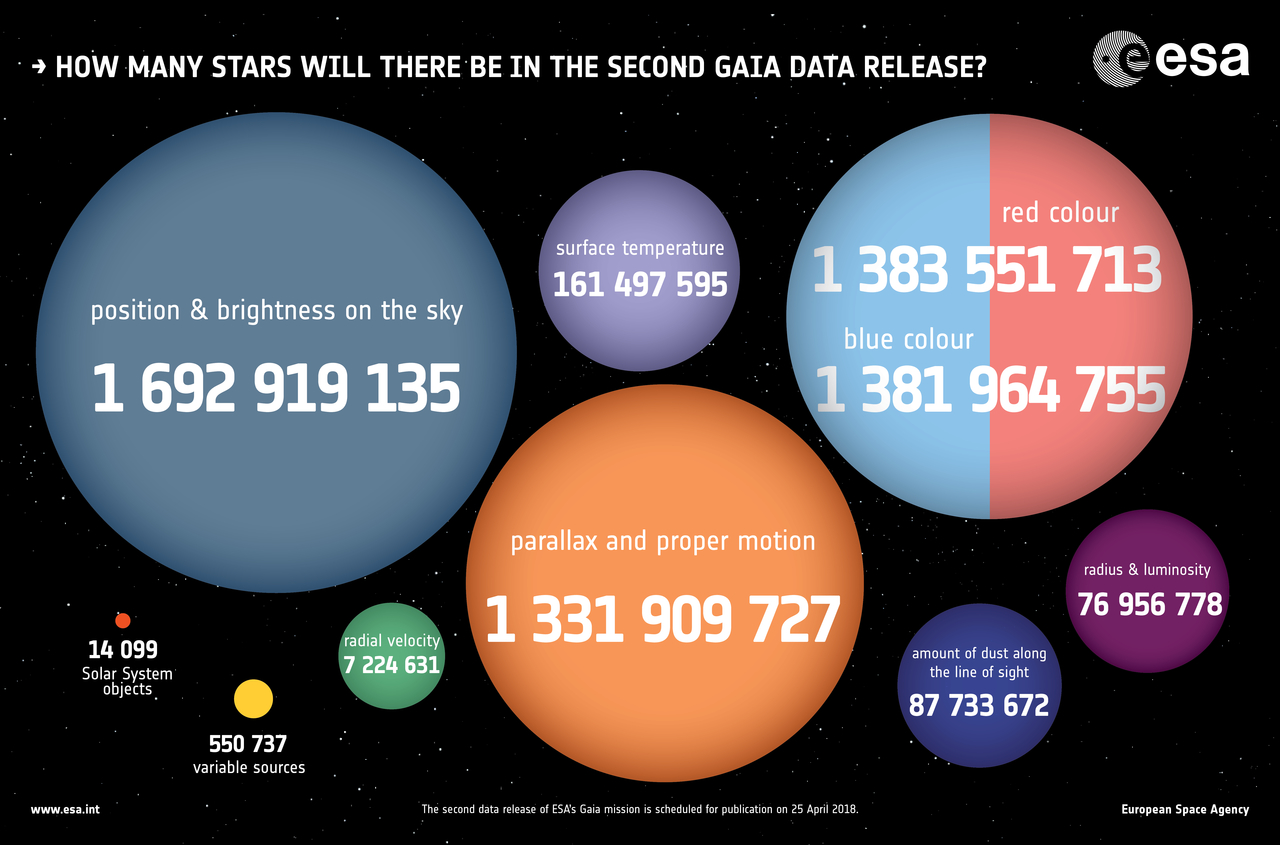
\includegraphics[width=\columnwidth]{1567214817936-Gaia_DR2_numbers_1280.jpg}
	\caption{Visual and numerical representation of \G\ DR2 stellar content. Image credit: ESA, CC BY-SA 3.0 IGO.}
	\label{fig:gaia_drs}
\end{figure}

Along the calibrated raw measurements, Gaia Data Processing and Analysis Consortium (DPAC) provides numerous parameters and properties of stars, pre-selected Solar system bodies and quasars that can be used and explored by users. Among them we can find:
\begin{itemize}
	\item \textbf{Astrometric set} consisting of partial 2-parameter (limited to celestial positions $\alpha$ and $\delta$) and full 5-parameter astrometric solution with addition of parallax, and proper motion in both coordinates. The 2-parameter sources are typically faint (with about half of them at magnitude G > 20.6), have very few observations (less than five as required for full solution), or very poorly fit the five-parameter astrometric model. All sources fainter than magnitude G = 21 have only positional information. In the current data release, all stars are still treated as a single during the astrometric fit, which could significantly influence solutions in the case of multiple fast-moving sources contributing to the position of an observed photocentre. The \G\ coordinate reference frame is aligned with the International Celestial Reference Frame (ICRF) using positions of extragalactic sources such as quasars \cite{2018A&A...616A..14G}. After the initial release, it was determined that the quality of an astrometric fit is best described by the astrometric re-normalised unit weight error (RUWE) \cite{ruwe}. The astrometric quality indicator RUWE is computed from the astrometric chi-squared goodness of fit and number of used observations that are both given in the published data table. To be comparable among stars of different absolute magnitude and colour, it was normalised by a factor given in the additional gridded data set. Normalising factors were produced by fitting the quadratic spline function to its non-normalised that depend on the stellar type and observed brightnesses. The most typical value of the parameter is one and can be as large as 50. Further details about astrometric processing and validation are given in \citet{2018A&A...616A...2L}, and \cite{2018A&A...616A...9L}.
	
	\item \textbf{Photometric data set} contains the broadband photometry in the G, G$_{BP}$, and G$_{RP}$ bands, giving us colour information for \G\ DR2 sources that were observed at least twice. The mean value of the G-band fluxes is reported for all sources while colour information (BP and RP) is available for about 80$\%$ of them.  The integrated colour information suffers from strong systematic effects at the faint end of the survey (G~>~$19$), in crowded regions, and near bright stars. In the case when measured fluxes are inconsistent between the G and the G$_{BP}$ and G$_{RP}$ bands (sum of the latter two is significantly larger than G measurement) a warning is raised. A quantitative index of this effect is provided in the numerical form as \textit{flux excess factor}. Further details about processing and photometry validation are given in \citet{2018arXiv180409368E}, and \cite{2018A&A...616A...3R}.
	
	\item \textbf{Radial velocity measurements} indicate stellar median radial velocity, averaged over the first 22 months of the observations. Distinct double-lined spectroscopic binaries were taken out from the list and will be published in later data releases. This filtering, to some degree, limits the possibility of finding multiple stars among observations. Some indication that a star could be part of a multiple system is unusually large velocity uncertainty. \G\ radial velocities are provided for sources which are brighter than magnitude 12 in the G$_{RVS}$ photometric band. A limited temperature range of the spectral template set which was used for the radial velocity determination implies that velocities are reported only for stars with effective temperatures in the range between $3550$ and $6900$~K (referring to the effective temperature of a used template and not an actual effective temperature of a star). By the RVS pipeline design, the determined absolute value of radial velocity is limited to within $1000$~\kms. The precision of the radial velocities at the faint end depend on stellar effective temperature and range from $1.4$~\kms\ for cooler to $3.6$~\kms\ for hotter stars. Those values indicate the typical spread of individual measurements during the observing period. The zero-point of the RVS velocities was determined using a comprehensive set of 4813 standard stars and asteroids with numerous dedicated, precise and temporally spread radial velocity measurements made at different observatories \cite{2018A&A...616A...7S}. Further processing details of RVS data are given in \citet{2018A&A...616A...6S}.
	
	\item \textbf{Stellar variability data set} consists of sources that were identified as photometrically variable (based on at least two photometric observations of the two \G\ telescopes). The final number still represents only a small subset of the total amount of variables expected in the \G\ survey. The sources were classified into the following nine categories based on their light curves: RR Lyrae (anomalous RRd, RRd, RRab, RRc), long-period variables (Mira type and Semi-Regulars), Cepheids (anomalous Cepheids, classical Cepheids, type-II Cepheids), $\delta$ Scuti and SX Phoenicis stars. If a star had 12 or more observations, its light curve was analysed in greater detail. They are designated as specific object studies (SOS) and consist of variables of the type Cepheid and RR Lyrae, long-period variables, short time scale variables, and rotational modulation variables. Full details on the variable star processing, results and their validation are given in \citet{2018A&A...618A..30H, 2018A&A...618A..58M, 2018A&A...620A.127M}, and \cite{2019A&A...622A..60C}.
	
	\item \textbf{Astrophysical parameters} derived by the astrophysical parameter inference system in the \G\ data processing (Apsis) include estimates of effective temperature \Teff, extinction A$_G$ and reddening E(G$_{BP}$~-~G$_{RP}$), radius, and luminosity for stars brighter than magnitude G~=~17. Values of \Teff\ are reported only over the temperature range between $3000$ and $10,000$~K Limits are induced by the training set of the algorithm responsible for the \Teff\ estimation. Estimates of the other astrophysical parameters are published for about half of the sources with determined \Teff. As the processing pipeline was performed individually for every object and with a limited set of input data (three \G\ photometric bands and parallax), some errors are expected because of high degeneracy between determined parameters. If a star is located far from expected isochrones used in the processing, extinction becomes overestimated and less usable for use. Full details of the astrophysical parameter processing and result validation are described in \citet{2018A&A...616A...8A}.	
	
	\item \textbf{Solar system objects} (SSO) data set provides epoch astrometry and unfiltered G photometry for a pre-selected list of $14,099$ known minor bodies in the solar system that are numbered in the Minor Planet Center repository. Each time a given SSO enters the field of view of \G\ telescopes, celestial positions are recorded as seen from the spacecraft. The data set and its production are thoroughly described in \citet{2018A&A...616A..13G}.
	
\end{itemize}

The above sections are partially adapted and summarized from \citet{2016A&A...595A...1G, 2018A&A...616A...1G}, and \cite{gaia_primer}.

\section{The GALAH survey}
\label{sec:galah_data}
The GALactic Archaeology with HERMES (GALAH, \cite{2015MNRAS.449.2604D}) is an ongoing spectroscopic survey that aims to unveil the Milky Way’s formation history by studying the detailed chemical composition of observed stars. As already explained in Chapter \ref{chap:intro}, the complete Galaxy did not form at the same time, but gradually over time. This formation history can be traced back by precisely determining the chemical composition of stars in its different regions. Remnants of initial building blocks, which have been disrupted during the formation and evolution, are now dispersed around the Galaxy. Chemical tagging theory \cite{2002ARA&A..40..487F} shows that those individual galactic components should have conserved their original chemical signature over time. It is therefore essential to disentangle their formation location and migration history in order to explain the current mixture of stellar populations. This component disentanglement can be achieved through the technique of chemical tagging that promises identification of old dispersed fossil remnants based on their unique abundance patterns over numerous chemical elements. The GALAH aims to achieve this by measuring up to 31 elemental abundances in every acquired spectrum. The observed elements come from seven independent major element groups with the different physical nucleosynthetic origin, which include light proton-capture elements Li, C, O; $\alpha$-elements Mg, Si, Ca, Ti; odd-Z elements Na, Al, K; iron-peak elements Sc,V, Cr, Mn, Fe, Co, Ni, Cu, Zn; light and heavy slow neutron capture elements Rb, Sr, Y, Zr, Ba, La; and rapid neutron capture elements Ru, Ce, Nd and Eu \cite{2015MNRAS.449.2604D}.

\begin{figure}
	\centering
	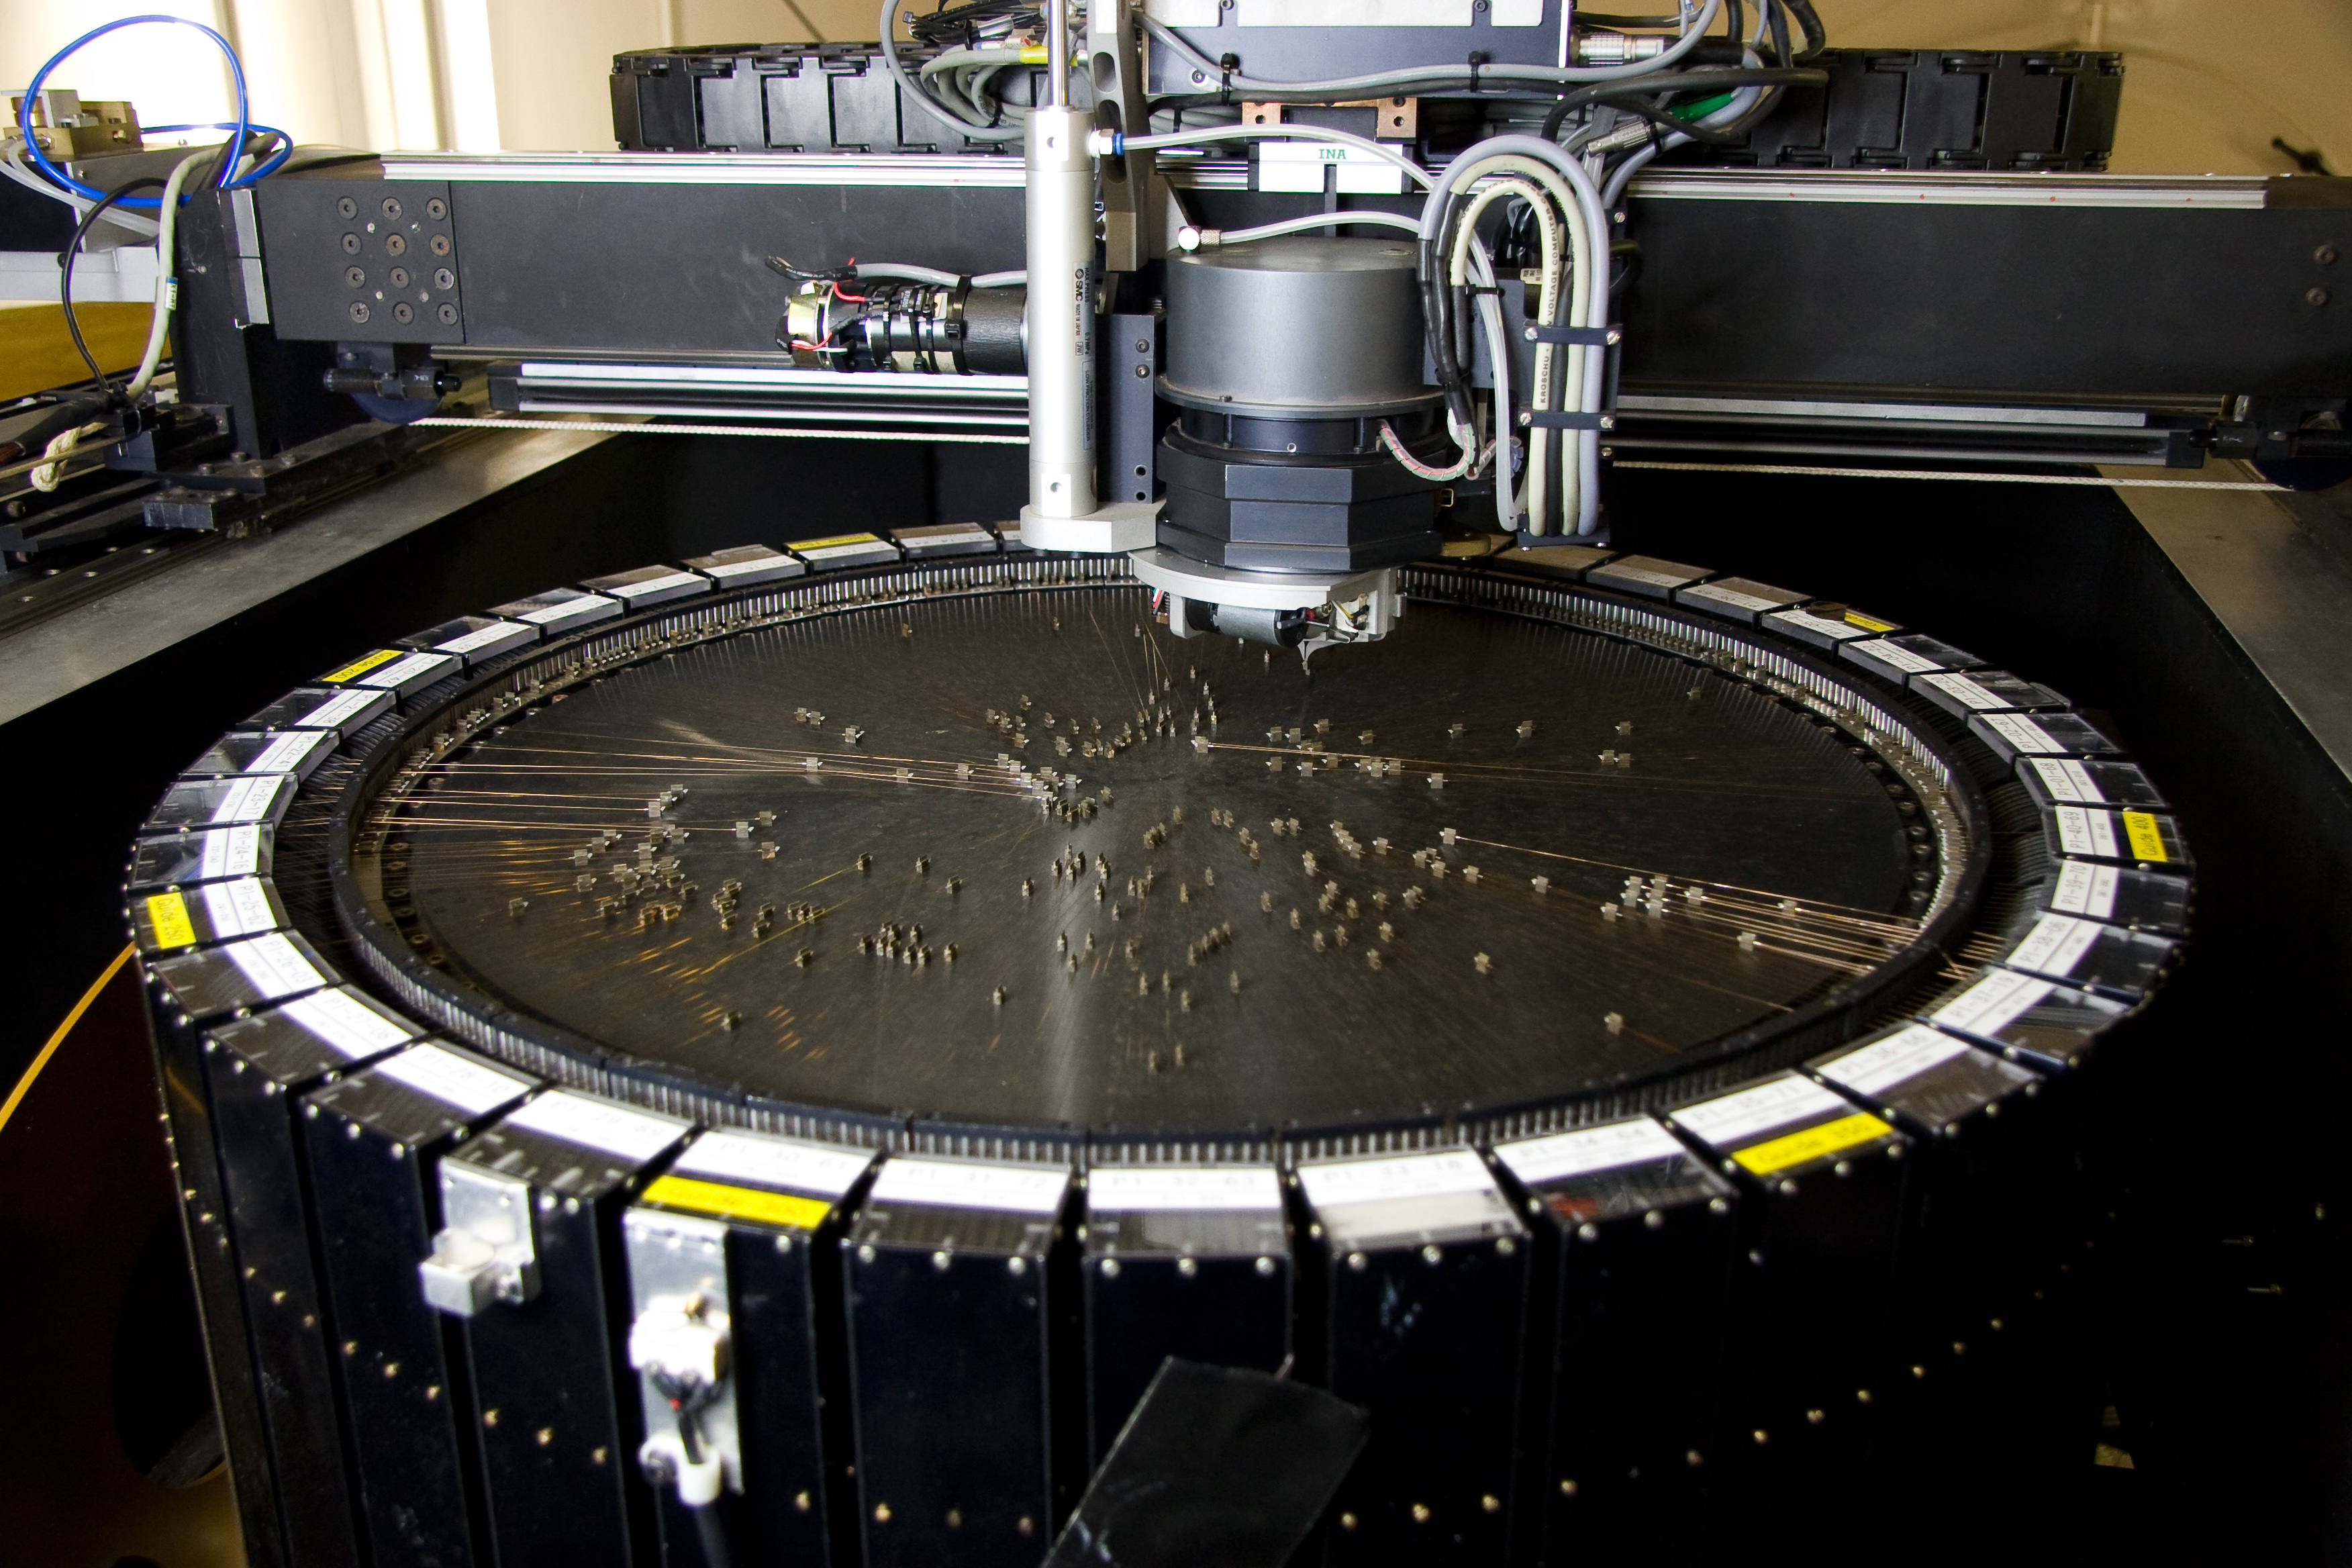
\includegraphics[width=0.48\columnwidth]{2df.jpg}
	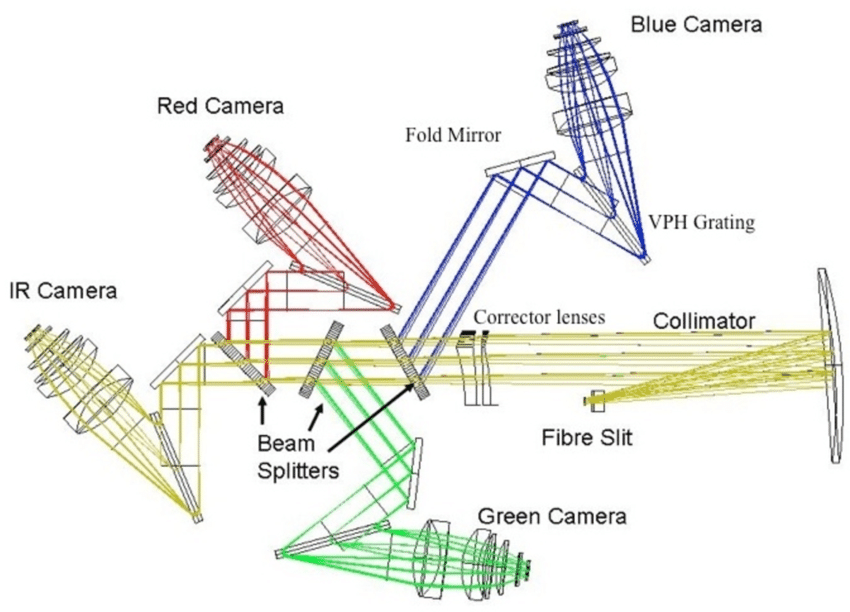
\includegraphics[width=0.48\columnwidth]{Optical-layout-of-the-HERMES-spectrograph.png}
	\caption{Crucial parts of the HERMES spectrograph are 2dF fiber positioner (left image) and four individual spectrograph arms.}
	\label{fig:hermes_2df}
\end{figure}

The GALAH survey was the main driver for the construction of the High Efficiency and Resolution Multi-Element Spectrograph (HERMES, \cite{2010SPIE.7735E..09B, 2015JATIS...1c5002S}), a multi-fibre spectrograph mounted on the $3.9$-metre Anglo-Australian Telescope (AAT) situated at the Siding Spring Observatory, Australia. The spectrograph has a resolving power of R $\sim 28,000$ (or R $\sim 45,000$ when slit mask is used) and covers four separately acquired wavelength ranges (4713 -- 4903~\AA, 5648 -- 5873~\AA, 6478 -- 6737~\AA, and 7585 -- 7887~\AA), together covering approximately 1000~\AA, including the H$\alpha$ and H$\beta$ lines. The ranges are frequently referred to as blue, green, red and near-infrared spectral arms (see left image of Figure \ref{fig:hermes_2df}). This configuration can simultaneously record spectra from up to 392 fibres distributed over a $2^\circ$ diameter field of the night sky, with an additional 8 fibres used for the telescope guiding. The fiber positioner has two identical plates that are used to precisely position fibers at designates stellar locations. During the exposure with the first plate, the robotic positioner is placing fibers on the second plate as shown in Figure \ref{fig:hermes_2df}. The complete fiber allocation process takes about half an hour per plate. The spectrograph can typically achieve a signal to noise ratio (SNR) $\sim100$ per resolution element at magnitude V=14 in the red arm during an 1-hour long exposure. To achieve as high SNR as possible and minimise atmospheric diffraction, all observations are ideally done when an observed field is passing through the meridian. With a fibers' finite field of view of 2\arcsec, we also want the object to be as high as possible on the sky. Observing at low altitudes could diffract different wavelengths over an angle that is larger than the fiber entrance point. Something that is not desigread as one of the spectrograph arms would receive less photons than others

\subsection{Acquired spectra and target selection}
The spectroscopic data used during the production of this thesis were taken from the pilot survey, the main GALAH survey \cite{2015MNRAS.449.2604D}, the K2-HERMES survey \cite{2018AJ....155...84W}, the TESS-HERMES survey \cite{2018MNRAS.473.2004S}, and specially dedicated the HEMRES open clusters (De Silva et al. in preparation) and the HERMES Orion star-forming region (Kos et al. in preparation) surveys. Together they form a dataset of $669,845$ successfully reduced stellar spectra, of which a small fraction belongs to repeated observations. All acquired spectra are homogeneously reduced to one-dimensional spectrum, normalised and shifted to the stellar reference frame (detailed description in \citet{2017MNRAS.464.1259K}). Combination of those surveys produces an increased number of spectra compared to the main GALAH survey. However, at the same time, this breaks the rule of a simple, unbiased selection function (Sharma et al. in preparation) that is desired for population studies and easier comparison with synthetic galactic models.

The original selection function of the main GALAH survey is separated into two magnitude limited field selections - bright (10<V<12) and regular (12<V<14) fields whose target selection is colour independent. Used V magnitude is inferred from magnitudes measured by the Two Micron All-Sky Survey (2MASS) \cite{2006AJ....131.1163S} whose photometric bands are shifted into the infra-red spectral region. Because of that, some, especially peculiar and variable stars, might have an erroneous estimation of V magnitude leading to underexposure or excessive spectral crosstalk. Because of expected crowding problems (projected diameter of used optical fibre on the sky is equal to $2$\arcsec) observed stars are located at higher Galactic latitudes ($|b|$~>~$10^\circ$) where the density of stars is lower. Additional surveys sometimes break those rules by selecting fainter/dimmer stars, going closer to the Galactic plane, employ colour cuts, or favour interesting preselected stars such as K2 \cite{2014PASP..126..398H} targets, TESS \cite{2015JATIS...1a4003R} targets and cluster members. Therefore some care is needed when trying to infer global stellar or galactic properties based on such inhomogeneous selection criteria.

\subsection{Spectral reduction and parameters determination}
The first step after recording spectra in the form of a 2D image is their extraction to multiple 1D spectra. The procedure, extensively documented by \citet{2017MNRAS.464.1259K}, consist of the following steps: raw image cosmetic corrections, spectral tracing, optical aberrations correction, scattered light and apertures cross-talk removal, wavelength calibration, sky subtraction, and telluric absorption removal. After reduction, spectra are normalised and shifted into their rest-frame by cross-correlating them with a set of 15 AMBRE model spectra \cite{2012A&A...544A.126D}. This procedure produces initial velocities that are usable for parameter determination, but not accurate enough for possible inter-cluster analysis. The more precise methodology uses the GALAH observations itself to compute a much denser set of reference spectra for cross-correlation. Its details are described by \citet{2018arXiv180406344Z}. In the last step, the methodology also accounts for gravitational redshift and convective blueshift to determine actual stellar radial velocity. 

Stellar atmospheric parameters and individual elemental abundances are in a uniform way derived from all normalised spectra. The applied parameter analysis pipeline slowly evolved and improved during the GALAH survey. The three most important milestones in an ongoing process are:

\begin{itemize}
	\item The initial stellar parameters (\Teff, \Logg, and \Feh), accompanying the first GALAH data release (\textbf{GALAH DR1}), were derived as a global fit (all arms at the same time) of the observed spectra to a grid of $16,783$ AMBRE spectra \cite{2012A&A...544A.126D}, which were convolved down to the average resolution of individual HERMES CCD. The aim of this procedure was to provide indicative stellar parameters, which could be used as a first initial guess to help speed up more complex stellar parameters and abundance pipelines.
	
	\item The parameters (with extension to \vsin, \vmic, and \aks) and up to 23 elemental abundances, released as part of the \textbf{GALAH DR2} \cite{buder2018}, were produced using the multi-step data-driven approach. The complete analysis depended on a set of $10,605$ spectra that were selected in such way to span a large portion of the parameter space and did not contain any peculiar star, especially binary and emission line spectra. Selected spectra were analysed using a physics-driven spectrum synthesis code Spectroscopy Made Easy (\SM, \cite{1996A&AS..118..595V, 2017A&A...597A..16P}) that performs spectrum synthesis for 1D stellar atmosphere models. In the case of DR2, it consists of MARCS theoretical 1D hydrostatic models \cite{2008A&A...486..951G} under the assumption of local thermodynamic equilibrium (LTE) for the majority of elements. The procure is computationally efficient but does not completely describe the physics inside stars. Therefore several vital elements (Li, O, Na, Mg, Al, Si, and Fe) were analysed using more realistic non-LTE line formation. A common approach to compute non-LTE abundances is to use the same pipeline as for LTE but internally account for the non-LTE departure coefficients that were in advanced computed using complex non-LTE computations that account for realistic atom collisions. Such departure coefficients are usually computed for a limited grid of stellar parameters and afterwards interpolated in between when need \cite{2020A&A...637A..80O, 2019A&A...630A.104A, 2020amarsigalah}.
	
	To propagate the parameter and abundance results of the training set to the whole survey, \TC\ \cite{2015ApJ...808...16N} generative data-driven approach was used. Here a crucial step is the preparation of the training set as it defines the quality of the employed machine learning procedure and consequently, quality and precision of the results. The training set was selected in such a way to span the stellar parameter ranges covered by stellar spectra completely. Therefore it mostly consists of well known and analysed stars, with many published results. Additionally, the set was cleared of any peculiarities (binary stars, fast rotators, reduction issues, etc.) that would introduce uncertainties into the learned model. Internally, \TC\ procedure adopts a simple quadratic model which uses stellar parameters to describe the observed flux of a given spectrum. Independent quadratic model is built for every spectrum wavelength bin. Flux at that bin is computed as a weighted linear combination of all possible two-parameter product combinations of input stellar parameters. To train \TC\ model, all the \Gh\ spectra in the training set were interpolated to a common wavelength grid. After the training was performed, the model was inverted to produce parameters and abundances for every observed spectrum. When a spectrum is introduced to an inverted \TC\ model, the latter tries to find the best matching stellar parameters. At every fitting step, \TC\ generates a learnt synthetic spectrum that is compared to the input spectrum. By minimising the difference between the generated and input spectrum, it tries to find the best matching parameters. Further details of the described process are given in \citet{buder2018}.
	
	\item Not relying on the GALAH spectral information alone, but including \G\ parallax, colour, and absolute magnitude, additional constraints and priors can be used to infer spectroscopic stellar parameters. That additional information can be used to confine information about \Logg\ and stellar age. Adaption of \SM\ software, thoroughly described in \citet{buder2020}, was used to accommodate additional \G\ information in order to produce the latest \textbf{GALAH DR3} data set. Unlike in DR2, no data-driven methodology was used to produce stellar parameters and abundances as \SM\ was run for every individual normalised spectrum. Reference spectra were generated using MARCS 1D stellar models. For eleven abundances (out of 30 measured) non-LTE corrections were performed. The published catalogue contains several additional Value-Added-Catalogues defining stellar ages and their galactic dynamics. To compute stellar masses and ages, the best matching PARSEC+COLIBRI isochrone was used.
	
	With the addition of so many auxiliary information with their own uncertainties, that are sometimes not even known or unable to be estimated, the question arises if they also impact the quality of the published results. As the precise parameters and abundances are the driving focus of the ongoing survey, we tried to estimate the possible trend and offsets by analysing open clusters in Chapter \ref{chap:clusters}.
	
\end{itemize}

\section{Asiago spectroscopic observations}
\label{sec:asiago_data}
Vastly different from the previous two massive all-sky surveys, telescopes at the Asiago site are mainly used for dedicated observations or monitoring of previously selected targets whose observational and astrophysical potential was identified from all-sky surveys. During our stay at the Asiago Observatory, that usually lasted for four consecutive bright nights (close to full Moon) every month, we used the $1.82$~m Copernico telescope located on top of the nearby hill Mount Ekar (Asiago, Italy - the altitude of $1,366$~m).

Our observations were performed by the Echelle spectrograph that is during near-full Moon days mounted on the telescope. At that time, the quality and deepness of photometric observations are heavily reduced and therefore not performed. Design of the Echelle instrument and its slit length enables the observer to observe only one star a time. Obtained spectra have a resolving power of R$\sim20,000$ and a wide span of wavelengths between $3600$ and $7400$ \AA. They are divided into 30 interference orders which partially overlap with succeeding and preceding order, providing an undisturbed coverage of observed wavelengths. Acquired spectra were recorded by the Andor DW436-BV CCD camera. The camera uses a back-illuminated CCD detector with a size of $2048 \times 2048$ pixels. This setup enables us to capture spectra of stars with magnitudes V~<~$10$ at high SNR with reasonable exposure time (less than 1 hour per spectrum). Because of the mechanical limitation, observed stars must be positioned at least $15^\circ$ above the local horizon. At those low altitudes, only the brightest stars are reasonable to be observed because of strong atmospheric attenuation and diffraction differences between red and blue wavelengths. The latter effect can be reduced by rotating the slit of the spectrograph into the paralactic angle.

Combining the location of the observatory and above observational limitations with the fact that our exciting stars were in advance selected from the GALAH survey, highly reduces the number of potentially observable objects. To reduce the atmospheric effects, we observed only stars which rose at least $30^\circ$ above the local horizon. This minimum altitude limitation is equal to omitting observable candidates as to having $\delta$~<~$-15^\circ$. As described in more detail below (see Chapters \ref{chap:peculiars_chem} and \ref{chap:twins}), we used additional Asiago observations to inspect spectroscopic features not accessible by the GALAH spectra and to prolong radial velocity time series of possible multiple stars who could show signs of radial velocity changes not detectable by a single epoch GALAH spectrum.

Additionally, to our program observations, we also contributed spectroscopic observations that resulted in published astronomer's telegrams \cite{2019ATel13340....1M} and scientific papers \cite{2019MNRAS.488.5536M}.

\begin{figure}
	\centering
	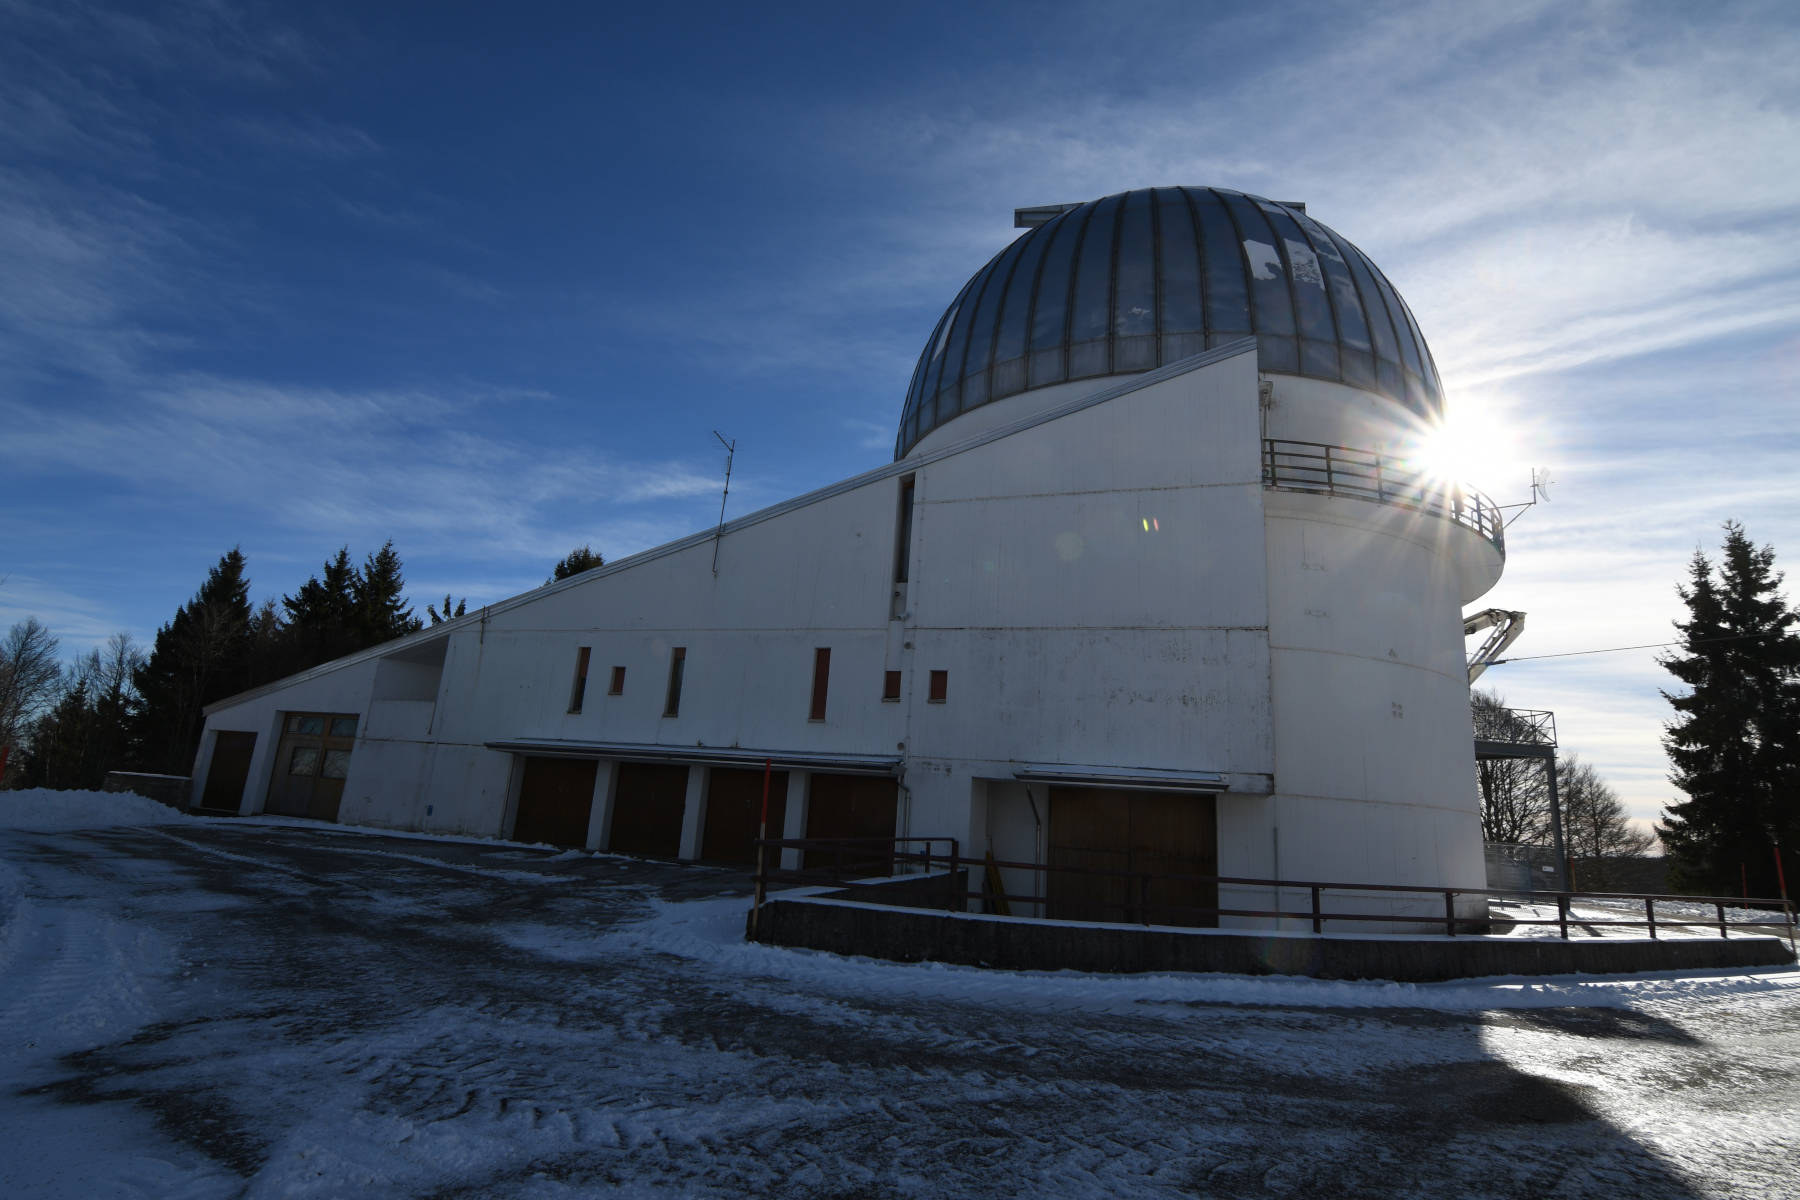
\includegraphics[width=0.8\textwidth]{DSC_8199.JPG}
	\caption{Structure and dome above the Copernico telescope on top the hill Mount Ekar, Asiago, Italy.}
	\label{fig:copernico_obs}
\end{figure}